Having established a means for Relative \pol{}, ensuring space and time synchronization within a zone, the next step would be to extend the protocol to finally achieve Absolute \pol{}. A possible path consists in combining the procedure with a Global Time Synchronization Protocol and a Global Positioning System, as illustrated in Figure~\ref{fig:proof-of-location-overview-absolute-pol}.

\begin{figure}[h!]
    \begin{center}
    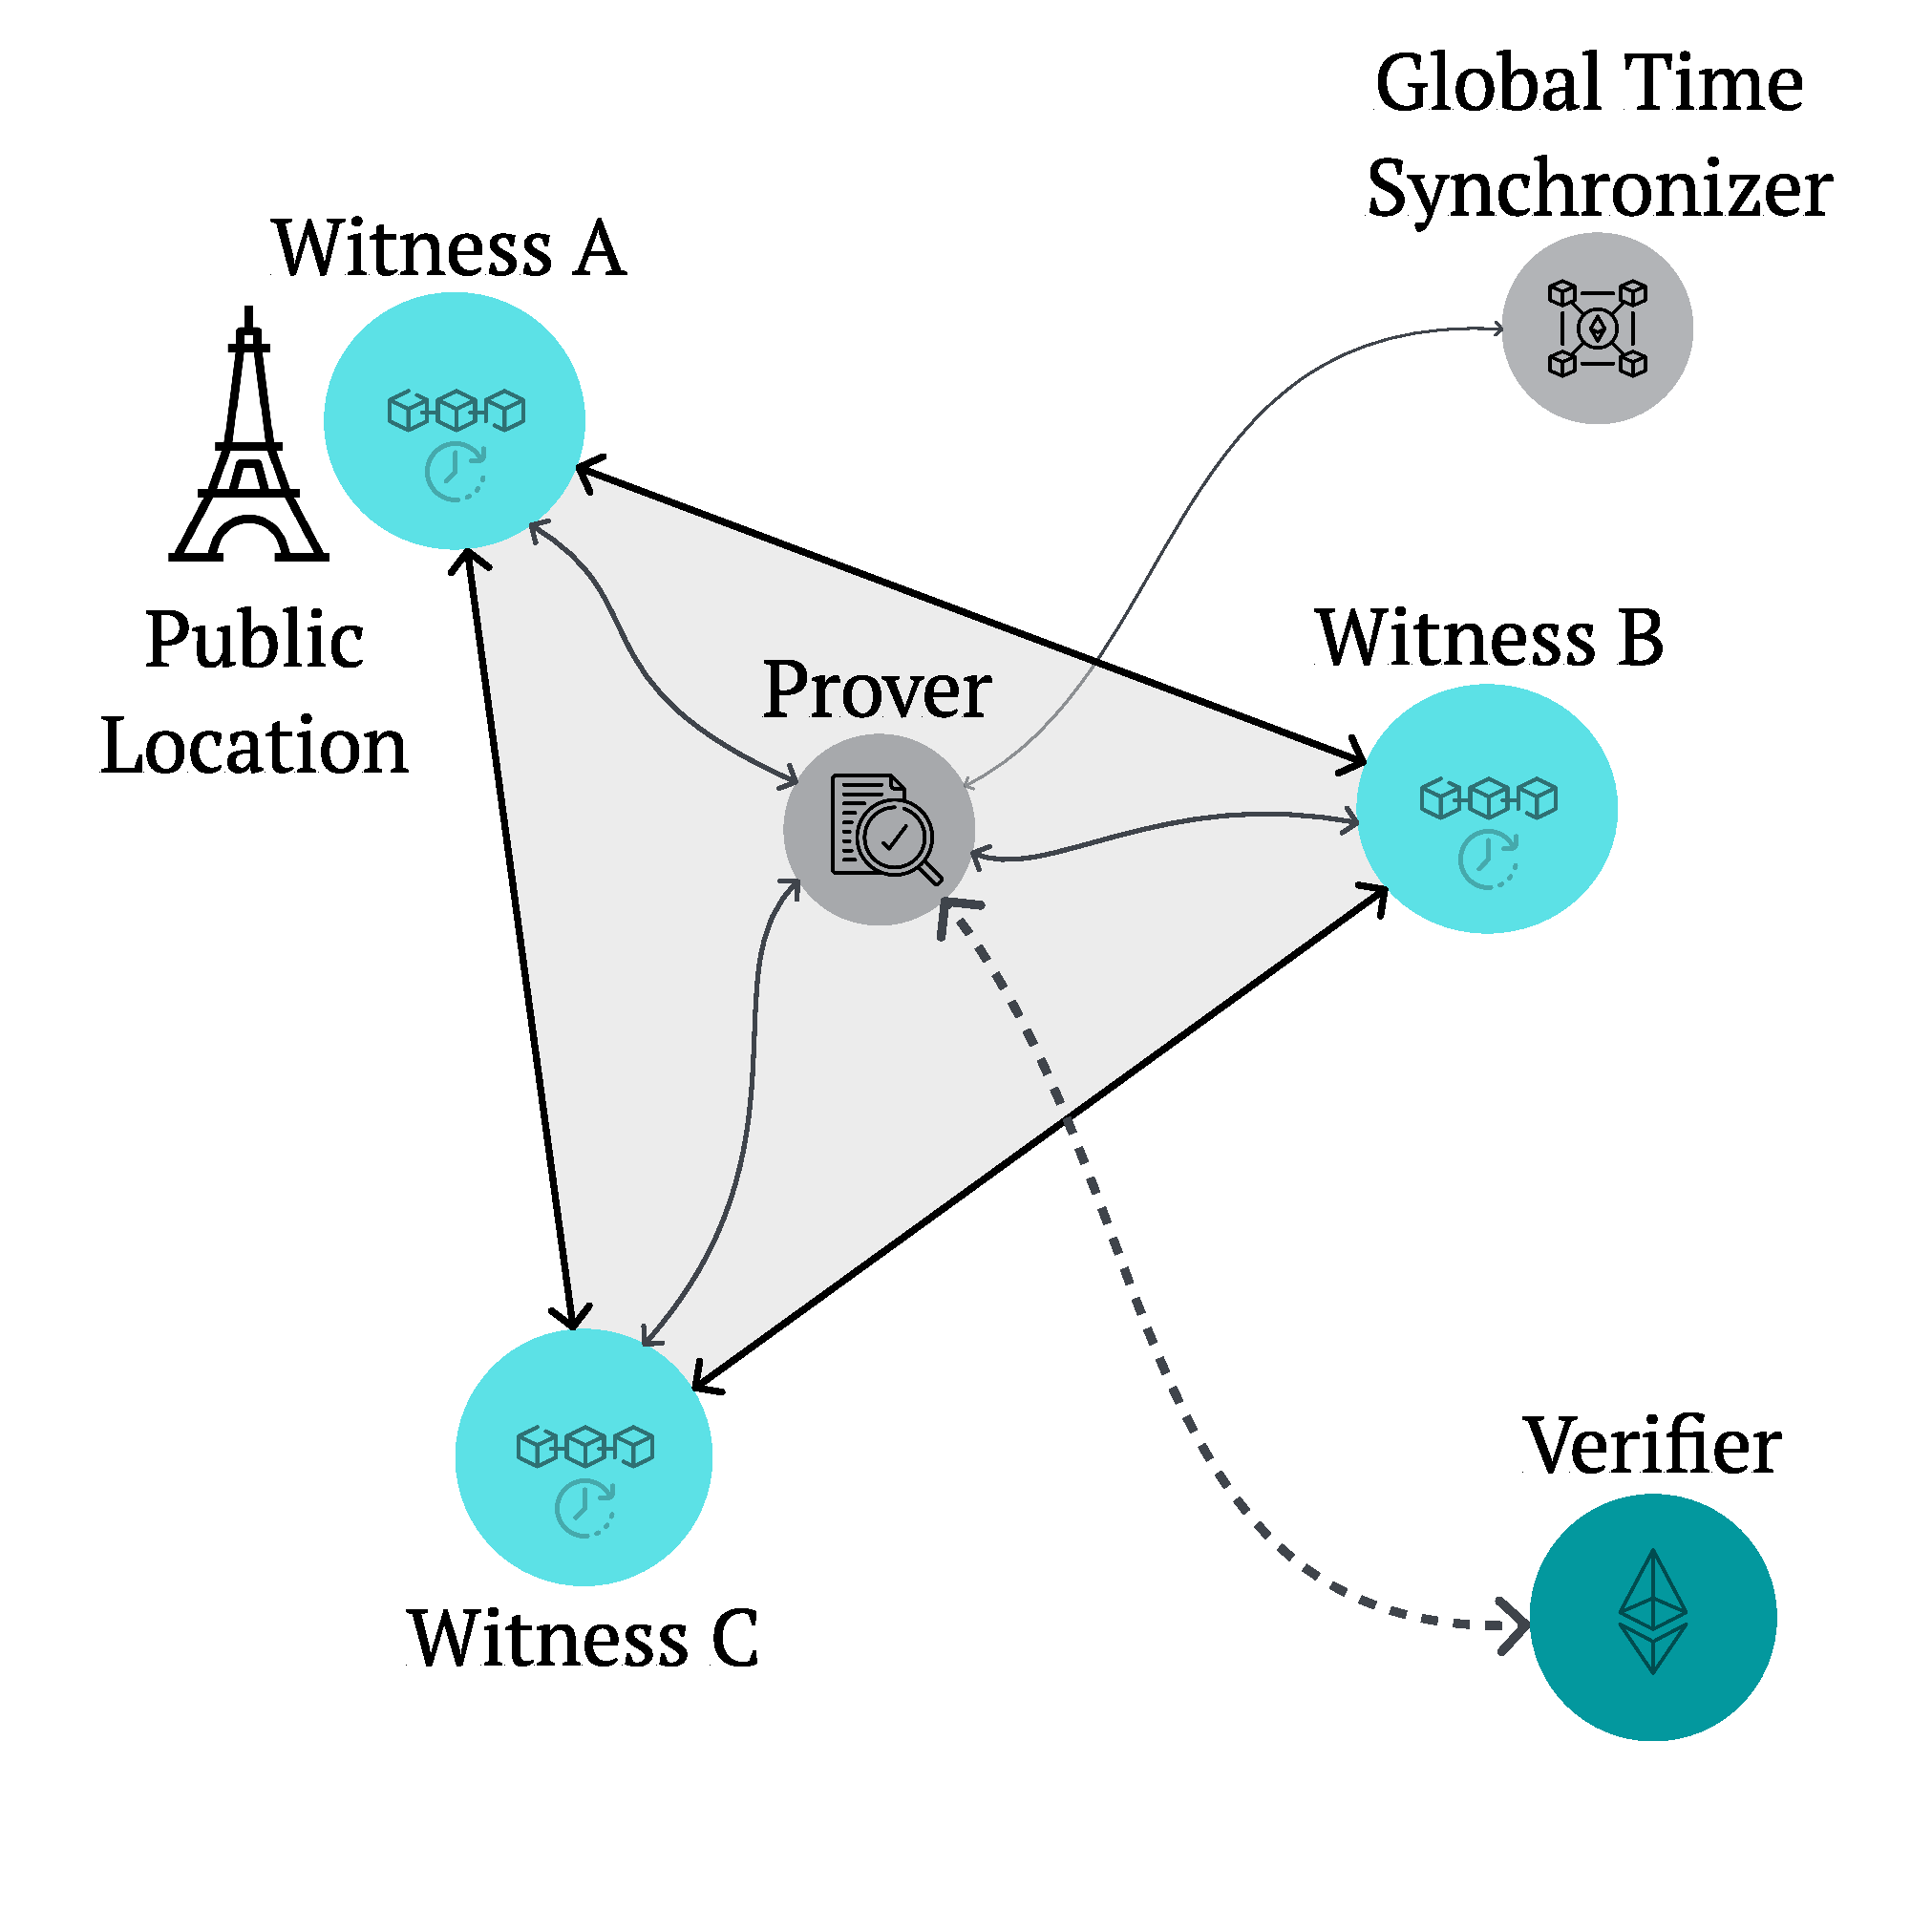
\includegraphics[width=0.55\textwidth]{overview-pol-abs-pol.pdf}
    \caption{Achieving Absolute \pol{} by combining Relative \pol{} with a Global Time Synchronization Protocol and a Global Positioning System.}
    \label{fig:proof-of-location-overview-absolute-pol}
    \end{center}
\end{figure}

The goal is to produce a \pol{} certificate that is spatio-temporally sound, relative to the zone, but which can, as well, be spatially and temporally acknowledged by any other node outside the zone. This effort may require, for instance, a global timestamping server, or protocol that can assert a certain level of globally secure timestamp accuracy in a tamper-proof manner. In a decentralized fashion, one example of such a system is a public Blockchain network, such as Bitcoin \cite{nakamoto2008bitcoin}, or Ethereum \cite{buterin2014next}. The same applies to the Global Positioning System (GPS). A standard system of geographic coordinates could be validated and embedded into the \pol{} certificate, to globally assert the location of the whole zone \cite{amoretti2018blockchain ,nosouhi2020blockchain}. It is worth noting that the Relative \pol{} protocol is flexible enough to accommodate any kind of higher level protocol, including more complex certificate formats, tighter trust levels, and composite information to be signed. This and further extensions are left for future work. \\

This chapter has laid the path towards a decentralized \pol{} protocol. We have started by proposing a mesh network topology to provide a decentralized and self-organizing network infrastructure. This underlying arrangement of nodes enables peer-to-peer and short-range communication, which is essential for the soundness of the protocol. Next, we have proposed a new way of synchronizing the internal clocks of trustless witnesses. This approach takes advantage of permissionless consensus mechanisms to establish zone-relative time consciousness and simultaneously enable the serialization of events in a tamper-proof manner. We have also considered the choice of a Turing-complete consensus system to allow for the decentralized execution of computations and deployment of zone-relative location services. Finally, we have proposed a \pol{} protocol that can produce a verifiable and spatio-temporally sound location certificate, relative to a zone. From Relative \pol{}, we are concluding the chapter with some thoughts on extending the protocol to achieve Absolute \pol{}.
